%%%%%%%%%%%%%%%%%%%%%%%%%%%%%%%%%%%%%%%%%%%%%%%%%%%%%%%%%%%%%%%%%%%%%%%%%%%%%%%%%%%%%%%%%%%%%%%%%%%%%%%%%%%%%%%%%%%%%%%%%%%%%%%%%%%%%%%%%%%%%%%%%%%%%%%%%%%
% This is just an example/guide for you to refer to when submitting manuscripts to Frontiers, it is not mandatory to use Frontiers .cls files nor frontiers.tex  %
% This will only generate the Manuscript, the final article will be typeset by Frontiers after acceptance.
%                                              %
%                                                                                                                                                         %
% When submitting your files, remember to upload this *tex file, the pdf generated with it, the *bib file (if bibliography is not within the *tex) and all the figures.
%%%%%%%%%%%%%%%%%%%%%%%%%%%%%%%%%%%%%%%%%%%%%%%%%%%%%%%%%%%%%%%%%%%%%%%%%%%%%%%%%%%%%%%%%%%%%%%%%%%%%%%%%%%%%%%%%%%%%%%%%%%%%%%%%%%%%%%%%%%%%%%%%%%%%%%%%%%

%%% Version 3.4 Generated 2018/06/15 %%%
%%% You will need to have the following packages installed: datetime, fmtcount, etoolbox, fcprefix, which are normally inlcuded in WinEdt. %%%
%%% In http://www.ctan.org/ you can find the packages and how to install them, if necessary. %%%

\documentclass[utf8]{frontiersSCNS}

%\setcitestyle{square} % for Physics and Applied Mathematics and Statistics articles
\usepackage{url,hyperref,lineno,microtype,subcaption}
\usepackage[onehalfspacing]{setspace}

\linenumbers


% BELOW TAKEN FROM rticles plos template
%
% amsmath package, useful for mathematical formulas
\usepackage{amsmath}
% amssymb package, useful for mathematical symbols
\usepackage{amssymb}

% hyperref package, useful for hyperlinks
\usepackage{hyperref}

% graphicx package, useful for including eps and pdf graphics
% include graphics with the command \includegraphics
\usepackage{graphicx}

% Sweave(-like)
\usepackage{fancyvrb}
\DefineVerbatimEnvironment{Sinput}{Verbatim}{fontshape=sl}
\DefineVerbatimEnvironment{Soutput}{Verbatim}{}
\DefineVerbatimEnvironment{Scode}{Verbatim}{fontshape=sl}
\newenvironment{Schunk}{}{}
\DefineVerbatimEnvironment{Code}{Verbatim}{}
\DefineVerbatimEnvironment{CodeInput}{Verbatim}{fontshape=sl}
\DefineVerbatimEnvironment{CodeOutput}{Verbatim}{}
\newenvironment{CodeChunk}{}{}

% cite package, to clean up citations in the main text. Do not remove.
\usepackage{cite}

\usepackage{color}

% Below is from frontiers
%
\bibliographystyle{frontiersinSCNS}
% Use doublespacing - comment out for single spacing
%\usepackage{setspace}
%\doublespacing


% Leave a blank line between paragraphs instead of using \\


\def\keyFont{\fontsize{8}{11}\helveticabold }


%% ** EDIT HERE **
%% PLEASE INCLUDE ALL MACROS BELOW

%% END MACROS SECTION


% tightlist command for lists without linebreak
\providecommand{\tightlist}{%
  \setlength{\itemsep}{0pt}\setlength{\parskip}{0pt}}


% Pandoc citation processing
\newlength{\cslhangindent}
\setlength{\cslhangindent}{1.5em}
\newlength{\csllabelwidth}
\setlength{\csllabelwidth}{3em}
\newlength{\cslentryspacingunit} % times entry-spacing
\setlength{\cslentryspacingunit}{\parskip}
% for Pandoc 2.8 to 2.10.1
\newenvironment{cslreferences}%
  {}%
  {\par}
% For Pandoc 2.11+
\newenvironment{CSLReferences}[2] % #1 hanging-ident, #2 entry spacing
 {% don't indent paragraphs
  \setlength{\parindent}{0pt}
  % turn on hanging indent if param 1 is 1
  \ifodd #1
  \let\oldpar\par
  \def\par{\hangindent=\cslhangindent\oldpar}
  \fi
  % set entry spacing
  \setlength{\parskip}{#2\cslentryspacingunit}
 }%
 {}
\usepackage{calc}
\newcommand{\CSLBlock}[1]{#1\hfill\break}
\newcommand{\CSLLeftMargin}[1]{\parbox[t]{\csllabelwidth}{#1}}
\newcommand{\CSLRightInline}[1]{\parbox[t]{\linewidth - \csllabelwidth}{#1}\break}
\newcommand{\CSLIndent}[1]{\hspace{\cslhangindent}#1}

\usepackage{natbib} % this is probably into you nips_2018 format file
\usepackage[T1]{fontenc}
% \usepackage{fontenc}
\usepackage{setspace}
\usepackage{siunitx}
\usepackage[customcolors,shade]{hf-tikz}
\usepackage{ragged2e}
% \usepackage[font=small,skip=0.25em,tableposition=top,figureposition=bottom]{caption}
\usepackage{amsmath}
\usepackage{mathtools}
\usepackage{etoolbox}
% \usepackage[skip=0.25em,tocskip=0.5em,indent=3em,parfill=0em]{parskip}
\usepackage{float}
\usepackage{array}
\usepackage{caption}
\usepackage{graphicx}
\usepackage{siunitx}
\usepackage{colortbl}
\usepackage{multirow}
\usepackage{hhline}
\usepackage{calc}
\usepackage{tabularx}
\usepackage{tabulary}
\usepackage{threeparttable}
\usepackage{wrapfig}
\usepackage{booktabs}
\usepackage{longtable}
\usepackage{array}
\usepackage{multirow}
\usepackage{wrapfig}
\usepackage{float}
\usepackage{colortbl}
\usepackage{pdflscape}
\usepackage{tabu}
\usepackage{threeparttable}
\usepackage{threeparttablex}
\usepackage[normalem]{ulem}
\usepackage{makecell}
\usepackage{xcolor}

\def\Authors{
  Issoufou Liman Harou\,\textsuperscript{1,2*},
  Julliet Inyele\,\textsuperscript{3},
  Lalisa Duguma\,\textsuperscript{1}}

\def\Address{

  \textsuperscript{1} Governance and Landscapes, World Agroforestry
(ICRAF),  Nairobi,  Nairobi,  Kenya
  
  \textsuperscript{2} Department of Environmental Sciences, Kenyatta
University,  Nairobi,  Nairobi,  Kenya
  
  \textsuperscript{3} Department of Geography, Kenyatta
University,  Nairobi,  Nairobi,  Kenya
  }

  \def\corrAuthor{Issoufou Liman Harou}\def\corrAddress{Kenyatta
University (KU)/ World Agroforestry (ICRAF)\\United Nations Avenue,
Gigiri\\Nairobi, Gigiri, P.O. Box
30677-00100 Kenya}\def\corrEmail{\href{mailto:issoufoul@gmail.com}{\nolinkurl{issoufoul@gmail.com}}}
  \def\firstAuthorLast{Liman Harou {et~al.}}
  
  
  
  


\begin{document}

\onecolumn
\firstpage{1}


\title[A spatial and temporal analysis of mangroves vegetation of The
Gambia]{A spatial and temporal analysis of mangroves vegetation of The
Gambia using seasonal metrics derived from times series of remotely
sensed data in Earth Engine}
\author[\firstAuthorLast]{\Authors}
\address{} %This field will be automatically populated
\correspondance{} %This field will be automatically populated

\extraAuth{}% If there are more than 1 corresponding author, comment this line and uncomment the next one.
%\extraAuth{corresponding Author2 \\ Laboratory X2, Institute X2, Department X2, Organization X2, Street X2, City X2 , State XX2 (only USA, Canada and Australia), Zip Code2, X2 Country X2, email2@uni2.edu}


\maketitle

\hypertarget{introduction}{%
\section*{Introduction}\label{introduction}}
\addcontentsline{toc}{section}{Introduction}

The Gambian mangroves, extending up to 160 km from the coast along the
River Gambia and covering an area ranging between 497 and 747 km2 , are
among the most developed mangroves of West Africa
(\protect\hyperlink{ref-Ajonina-et-al-2013}{Ajonina et al., 2013};
\protect\hyperlink{ref-Feka-and-Ajonina-2011}{Feka and Ajonina, 2011};
\protect\hyperlink{ref-Spalding-et-al-1997}{Spalding et al., 1997}). In
The Gambia, mangroves provide fish, oysters, shrimps, wood fuel, and
timber for construction along with many other ecosystem services to the
coastal inhabitants (\protect\hyperlink{ref-Ceesay-et-al-2017}{Ceesay et
al., 2017};
\protect\hyperlink{ref-Satyanarayana-et-al-2012}{Satyanarayana et al.,
2012}; \protect\hyperlink{ref-UNEP-2007}{UNEP, 2007}).There is a need to
monitor the use of these mangroves for sustained provisioning of the
services they provide
(\protect\hyperlink{ref-Satyanarayana-et-al-2012}{Satyanarayana et al.,
2012}).

Despite the importance of these ecosystems for the Gambian communities,
the current trend of mangroves vegetation in The Gambia remains unclear.
The interpretations of mangroves dynamics in the region diverge because
the scale of most remote sensing analysis do not always capture local
accounts of destruction (\protect\hyperlink{ref-Fent-et-al-2019}{Fent et
al., 2019}). \protect\hyperlink{ref-Spalding-et-al-1997}{Spalding et
al.} (\protect\hyperlink{ref-Spalding-et-al-1997}{1997}) reported a
decrease from 600 to less than 500 km2 between 1982 and 1995.
\protect\hyperlink{ref-UNEP-2007}{UNEP}
(\protect\hyperlink{ref-UNEP-2007}{2007}) reported a slight decrease in
mangroves vegetation and attributed it to drought, increase in soil
salinity, illegal exploitation and land use conversion.
\protect\hyperlink{ref-Ceesay-et-al-2017}{Ceesay et al.}
(\protect\hyperlink{ref-Ceesay-et-al-2017}{2017}) estimated this decline
in Tanbi Wetlands National Park of The Gambia at 6\% between 1973 and
2012 and attributed it to increase salinity which negatively affect
mangrove regrowth and rejuvenation. In Central River region of The
Gambia, \protect\hyperlink{ref-AliBah-2019}{Ali Bah}
(\protect\hyperlink{ref-AliBah-2019}{2019}) estimated this decline at
5.54\% between 1984 and 1994, 7.18\% between 1994 and 2007 and 22.02\%
between 2007 and 2017 and attributed it to increase temperature and
decrease in rainfall. In contrast, Fent et al.
\protect\hyperlink{ref-Fent-et-al-2019}{Fent et al.}
(\protect\hyperlink{ref-Fent-et-al-2019}{2019}) found an overall
increases in mangrove vegetation areas of 51.21\% between 1988 and 2018
across The Gambia and in the Sine Saloum and lower Casamance estuaries
in Senegal. In these areas, mangroves have seen important recovery
between 1988 and 1999 following the increased precipitation and tree
species regrowth that experiences diebacks due to salinisation caused by
drought (\protect\hyperlink{ref-Fent-et-al-2019}{Fent et al., 2019}). It
is clear from these studies that mangroves dynamics is a complex topic
that require multi-disciplinary approaches where various scale-dependent
factors are required. Evidence from recent studies
(\protect\hyperlink{ref-Fent-et-al-2019}{Fent et al., 2019}) have shown
that neither climatic, nor political, nor anthropogenic factors alone
can explain the dynamic of mangroves vegetation near the Gambia, and
arguably elsewhere. While Sine Saloum experienced lower precipitation
increase between 1988 and 1999 compare to Low Casamance, the former have
seen an important increase and the latter a slight decline in mangrove
vegetation (\protect\hyperlink{ref-Fent-et-al-2019}{Fent et al., 2019}).

Perhaps, the reasons for these discrepancies in estimates can be
explained by the sporadic nature of the available studies which targeted
different period and scale of analysis. In our knowledge, none of these
studies succeeded in fully reconstructing the time series of satellite
images due to various remote sensing artifacts in the region and
limitations in computing resources for handling big data. With few
exceptions (\protect\hyperlink{ref-Fent-et-al-2019}{Fent et al., 2019}),
studies aiming at The Gambian mangroves have not been sufficiently
holistic in the sense of explaining the dynamics of the biophysical
settings in their specific context. Most the available estimates of
mangroves areas and trends in The Gambia used single point images
classification approaches in an image differencing framework. Many
problems can arise. Because mangroves can be easily confused with other
ecological systems (e.g.~forests), studies aiming to provide realistic
estimates of mangroves dynamics should accurately account for spatial
and temporal variability of coastal ecosystems
(\protect\hyperlink{ref-Fent-et-al-2019}{Fent et al., 2019}).

The objective of this study is to assess mangrove extent dynamics in The
Gambia. We used locally continuous time series of remotely sensed images
to map all major land use and land cover (LULC) while putting emphasis
on mangrove vegetation dynamics in the Gambia.

\hypertarget{materials-and-methods}{%
\section*{Materials and methods}\label{materials-and-methods}}
\addcontentsline{toc}{section}{Materials and methods}

\hypertarget{ref22}{%
\subsection{Definition of key terms}\label{ref22}}

In this section, we define several terms which may lead to confusion.
Remote sensing artifacts regroup all atmospheric (e.g., such as cloud,
cloud shadow, haze, aerosol scattering) and technical factors (e.g.,
scan line corrector failure in Landsat 7 Enhanced Thematic Mapper Plus)
that would potentially lead to unrealistic pixel value estimates. The
term ``clear'' (as in clear pixels or clear observation) is meant for
pixels exempt of any remote sensing artifacts. We used the term
``cloudy'' (as in cloudy observations or cloudy pixels) to denote pixel
value identified by Fmask algorithm as affected by remote sensing
artifacts. These are different from ``noisy'' (as in noisy observations)
which are to be understood as clear pixel whose values are not
reasonably within the range of valid values. These are mostly cloudy
pixels not identified by Fmask algorithm. We used the term ``signal'' to
denote the smooth temporal distribution of pixel values that describes
the average phenological profile at the pixel. This is the information
of interest as opposed to ``noise'' which denotes the random
fluctuations that obscures the signal.

\hypertarget{ref21}{%
\subsection{Study area}\label{ref21}}

The study area, The Gambia (Figure \ref{fig:fig1}), is located on the
Gulf of Guinea, bordered by the Atlantic Ocean to west while forming an
enclave within Senegal. The country occupies an area of 10,689 km2
extending 320 km along Gambia river. As of 2013, the population of The
Gambia is estimated at 1.9 million with a growth rate of 3.3\% per annum
(\protect\hyperlink{ref-TheGambiaBureauofStatistics-2013}{The Gambia
Bureau of Statistics, 2012}). The prevailing climate is of type Sudan
Sahelian with an average annual rainfall of around 900 mm, a mean
temperature near 25°C, a long dry season between November to May and a
rainy season between June to October. Gambia river is perhaps the most
visible feature of The Gambia with its densely continuous tickets of
mangroves that represent a valuable shelter for diverse species
(\protect\hyperlink{ref-Spalding-et-al-1997}{Spalding et al., 1997}).

\begin{figure}
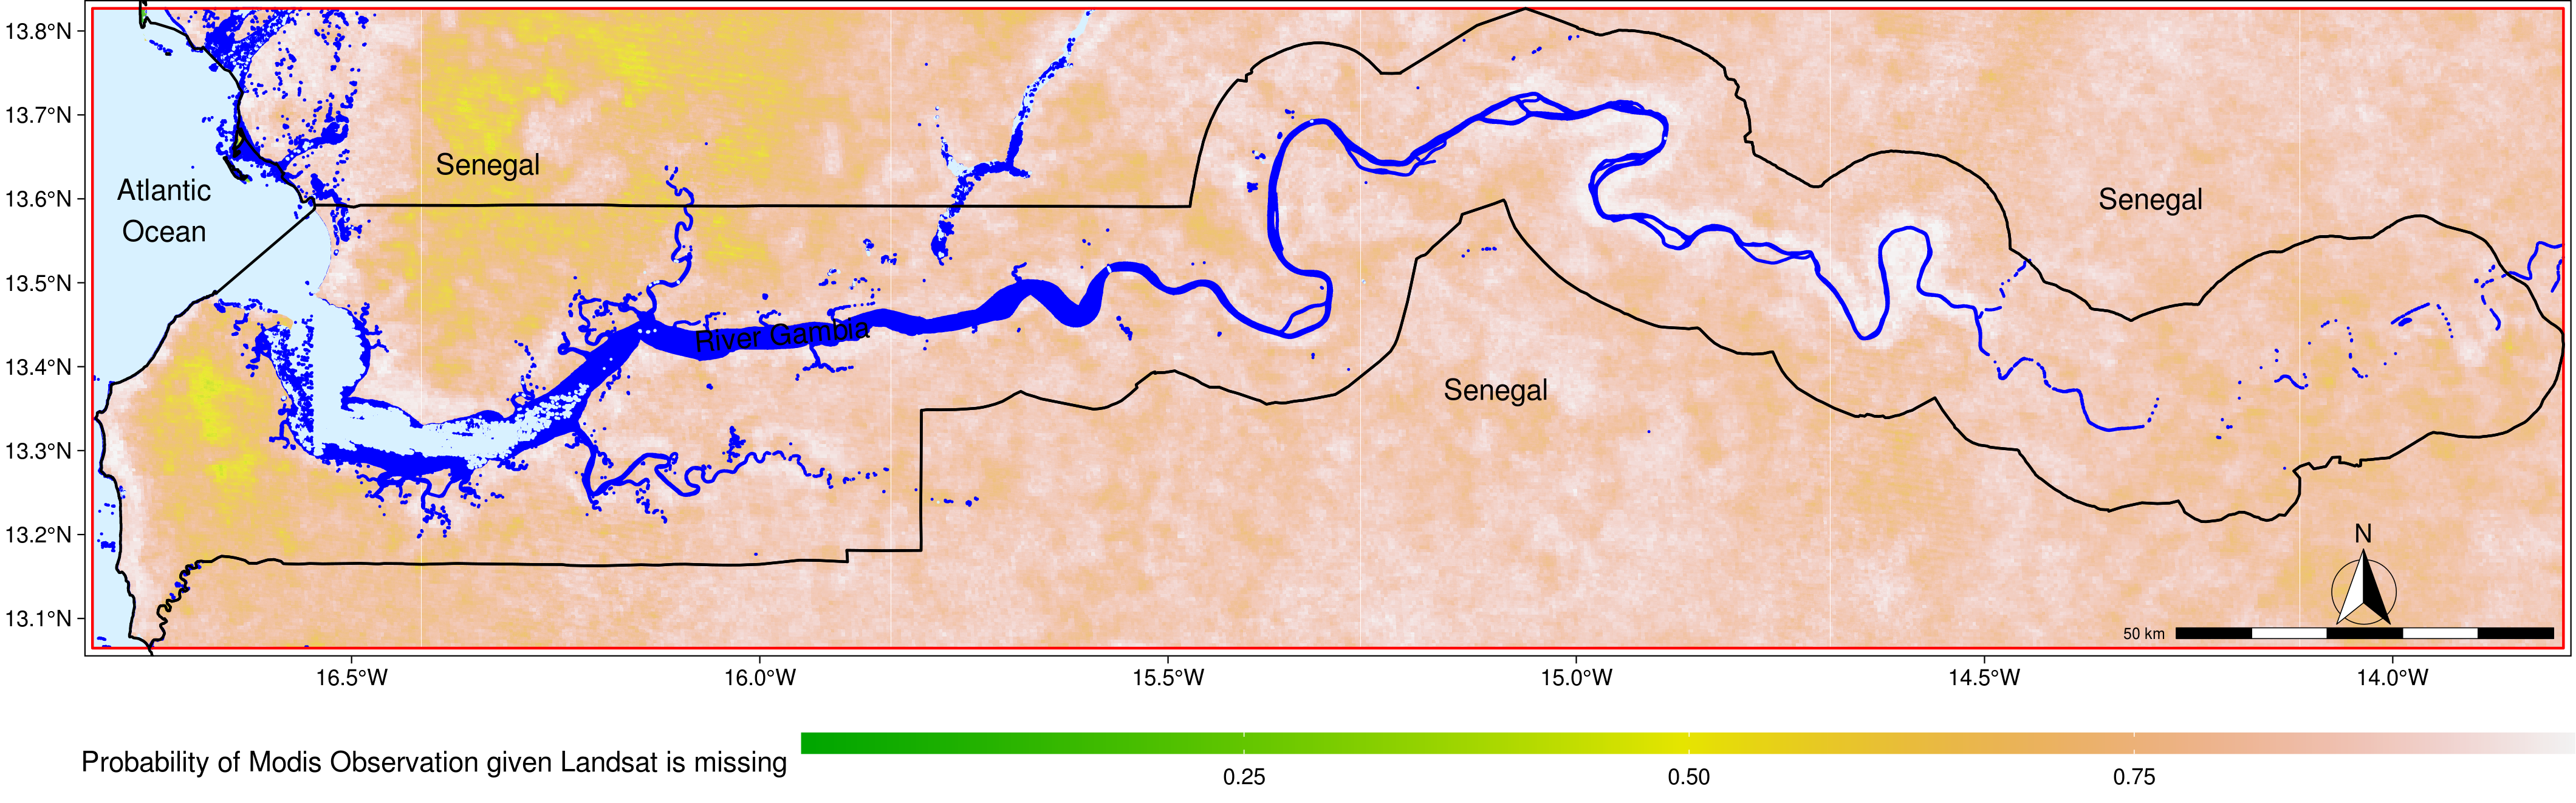
\includegraphics[width=1\linewidth]{figures/Gambia_study_area_map} \caption{Delineating the referential area for the analysis.}\label{fig:fig1}
\end{figure}

For reference data, we considered the rectangular area enclosing the
country to include all mangroves. The Gambian mangroves have been the
center of important debates - mangrove regrowth versus mangroves
degradation - over the last few decades. The Gambia has a reach body of
LULC (e.g., water bodies, forests, savannas, shrublands, croplands),
most of which are strongly influenced by the prevailing anthropogenic
and ecological processes taking place in the coastal regions
(\protect\hyperlink{ref-Andrieu-2018}{Andrieu, 2018}).

\hypertarget{ref23}{%
\subsection{Satellite imageries}\label{ref23}}

To provide accurate estimates of mangroves in The Gambia, the present
study considered all Landsat Tiers 1 and MODIS MOD09A1 V6 collections
available from Google Earth Engine cloud computing platform
(\protect\hyperlink{ref-Gorelick-et-al-2017}{Gorelick et al., 2017};
\protect\hyperlink{ref-Vermote-2015}{Vermote, 2015};
\protect\hyperlink{ref-Wulder-et-al-2019}{Wulder et al., 2019}). These
account for 2,916 Landsat and 959 MODIS tiles (used for filling gaps in
Landsat data) of land surface reflectance data spread across 3 bands
(i.e., visible red, near infrared and shortest wave infrared) acquired
between the years 2000 and 2020. The atmospherically corrected Landsat
and MODIS surface reflectance provide reasonable estimates of target
reflectance as it would be measured on the ground, making them good
candidates for LULC analysis. The main artifact that influences the
usefulness and usability of these images in the study area is the
important cloud coverage during the rainy season.

\hypertarget{ref24}{%
\subsection{Referential for data and image classification}\label{ref24}}

We conducted extensive field survey to systematically collect reference
data for training and validation of LULC classification. These training
and validation polygons, collected following the guidelines and class
definition of the international geosphere -- biosphere program
(\protect\hyperlink{ref-FRA-2000}{FRA, 2000}) and the FAO land cover
classification System (\protect\hyperlink{ref-Di-Gregorio-et-al-2016}{Di
Gregorio et al., 2016}), are fairly evenly distributed across the major
LULC in the region. We covered 15 different classes (Table
\ref{tab:tab1}) valid for the 3 reference periods considered for LULC
classification. Considering that land use and cover change in the study
areas are mostly gradual and hoping to capture the essential
intra-annual changes over a relatively short period (3 years), our
reference periods are 2000 to 2002, 2010 to 2012 and 2018 to 2020. We
will refer to these as 2000, 2010 and 2020 and their respective
classifications as 2000-classification, 2010-classification and
2020-classification. By considering multiple years, hence deriving land
use and cover classification over a period, we minimized the chances of
capturing noise, because LULC changes due to noise tend to be ephemeral
whereas true land cover changes tend to persist through time
(\protect\hyperlink{ref-Zhu-and-Woodcock-2014}{Zhu and Woodcock, 2014}).

To account for the spatial distribution of LULC in relation to the
reflectance values in the image time series, we constrained the training
and validation data to areas whose classes have not changed between the
reference periods, given the spatial and temporal distribution of the
surface reflectance values. We used k means clustering to produce
unsupervised classifications (15 classes distributed over 1000 random
points) for both reference periods based on which we conducted a
stratified random sampling across those locations whose LULC remain
unchanged. This required careful visual observation and matching of
class configurations across the entire landscapes of the classified
images. While this process was tedious and time consuming, it helped us
to produce classifiers that are consistent with both reference periods.
For each class (Table \ref{tab:tab1}), we considered 500 samples, making
a total of 7500 points, to train and validate a model for land use and
land cover classification.

\begin{table}[H]

\caption{\label{tab:tab1}Categories of land use and land cover used for an image classification in The Gambia.}
\centering
\resizebox{\linewidth}{!}{
\begin{threeparttable}
\begin{tabular}[t]{llr}
\toprule
\textbf{Standard class} & \textbf{Class description} & \textbf{Map legend}\\
\midrule
Fresh water & Lakes, rivers, and other reservoirs that are dominantly freshwater bodies. & Fresh waters\\
\addlinespace
Salty water & Oceans, seas and other reservoirs that are dominantly salty water bodies. & Salty waters\\
\addlinespace
Closed forests & Lands dominated by trees with a percent cover greater than 70 \% during the entire period of the year. & Closed forests\\
\addlinespace
Open forests & Lands dominated by trees with a percent cover between 60 and 70 \% during the entire period of the year. & Open forests\\
\addlinespace
Woody savannas & Lands with herbaceous and other understory systems, and with forest canopy cover between 30\% and 60\%. The forest cover height exceeds 2 m. & Woody savannas\\
\addlinespace
Savannas & Lands with herbaceous and other understory systems, and with forest canopy cover between 10\% and 30\%. The forest cover height exceeds 2 m. & Savannas\\
\addlinespace
Closed shrublands & Lands with woody vegetation less than 2 m tall and with shrub canopy cover > 60\%. The shrub foliage can be either evergreen or deciduous. & Closed shrublands\\
\addlinespace
Open shrublands & Lands with woody vegetation less than 2 m tall and with shrub canopy cover between 10\% and 60\%. The shrub foliage can be either evergreen or deciduous. & Open shrublands\\
\addlinespace
Grasslands & Lands with herbaceous types of cover. Tree and shrub cover is less than 10\%. & Grasslands\\
\addlinespace
Permanent wetlands & Lands with a permanent mixture of fresh water and herbaceous or woody vegetation. & Wetlands\\
\addlinespace
Croplands & Lands covered with temporary crops followed by harvest and a bare soil period (e.g., single and multiple cropping systems). Perennial woody crops are classified as the appropriate forest or shrub land cover type. & Croplands\\
\addlinespace
Urban and built-up lands & Land covered by buildings and other man-made structures. & Built-up\\
\addlinespace
Cropland / natural vegetation mosaics & Lands with a mosaic of croplands, forests, shrubland, and grasslands in
which no one component comprises more than 60\% of the landscape. & Mosaics\\
\addlinespace
Barren & Lands with exposed soil, sand, rocks, or snow and never have more
\textbf{than 10\% vegetated cover during any time of the year.} & \textbf{Barren}\\
\addlinespace
Mangroves & Lands with a permanent mixture of salty or brackish water and herbaceous or woody vegetation. & Mangroves\\
\addlinespace
Regularly Flooded Vegetation & Land transitioning between terrestrial and fresh water zones with sufficient moisture for the development of near evergreen vegetation. & Riperian Vegetation\\
\bottomrule
\end{tabular}
\begin{tablenotes}
\item \textit{Note: } 
\item Fresh and salty water, based on the definition of class water bodies in IGBP land cover classification system, are considered to capture the reach of fresh and salty water as this can be relevant in the context of mangrove ecosystems. Closed and opened forests are based on FAO LULC classification system. The remaining class are based on IGBP land cover classification system.
\end{tablenotes}
\end{threeparttable}}
\end{table}
\vspace{-2em}

\renewcommand{\arraystretch}{0.25}

This study involved a systematic review of the existing literature aimed
to mangrove ecosystems in The Gambia and neighboring areas as well as a
remote sensing-based analysis of mangroves change using continuous time
series. Our approach for change detection unravels several mysteries
surrounding the topic to address several shortcomings regarding LULC
analysis in The Gambia and can provide clues for accurate LULC analysis
elsewhere. It involved several steps for data scaling and gaps filling
to minimize the effects of sensors difference (e.g., Landsat ETM+ versus
Landsat OLI) and remote sensing artifacts (e.g., clouds, and cloud
shadows) along with a temporal smoothing to remove random noise.

\hypertarget{ref31}{%
\subsection{Image pre-processing}\label{ref31}}

As mentioned earlier, we used the geometrically and atmospherically
corrected Landsat surface reflectance products. These products are
provided along with a quality assessment band which we used to mask all
pixels affected by remote sensing artifacts. Although these are
currently amongst the best available Landsat and MODIS products in the
public domain, they often need to be further processed prior to analysis
involving continuous observations. Since the atmosphere correction may
fail to account for these remote sensing artifacts
(\protect\hyperlink{ref-Zhu-and-Woodcock-2014}{Zhu and Woodcock, 2014}),
we discarded all pixels but those acquired under clear conditions. In
the few cases where no clear acquisition is available, we created an
empty image to keep track of missing data and provide a slot for gap
filling, which we conducted in 3 steps. Roy et al.
\protect\hyperlink{ref-Roy-et-al-2016}{Roy et al.}
(\protect\hyperlink{ref-Roy-et-al-2016}{2016}) noted differences between
OLI and others Landsat data and provided coefficients for harmonizing
these using linear transformation. We scaled all data from other sensors
to OLI, so that the time series can be comparable over the 20 years.
This is particularly important for studies using water or vegetation
indices because the difference is higher in the near infrared and short
wave infrared bands whereas atmospheric correction increases this
difference in the visible bands
(\protect\hyperlink{ref-Roy-et-al-2016}{Roy et al., 2016}).

\begin{figure}
\includegraphics[width=1\linewidth]{figures/Gambia_ndsi_ts} \caption{Available monthly median Landsat NDVI and NDWI values after MODIS gap filling (red points), and their corresponding predicted values (green lines) estimated using harmonic modelling at different location in The Gambia. This figure illustrates how the model fits to different data inputs to capture variations across multiple pixels.}\label{fig:fig2}
\end{figure}

The first step for gap filling consisted in computing the monthly median
composites, considering a lag of 31 days. This reduced the number of
images to 12 medians images per year, corresponding to 1 image per
month. The median has proven to be a robust statistic in the sense that
it is tolerant to outliers and noisy observations.

In the second step, we used the median of the corresponding MODIS
acquisition of the month to fill data gaps in the Landsat composite
where these MODIS data are available. We then computed the normalized
difference vegetation (NDVI) and water (NDWI) indices, which we used for
subsequent analysis. The use of these indices can also improve the
accuracy in data estimates since values beyond the range {[}-1, 1{]} are
systematically discarded. The choice of these two spectral indices is
motivated by their sensitivity to water and vegetation, which are
sufficient to describe the landscape of the study area when times series
are available. The third step exploit the vegetation and water
seasonality in the study region, hence the temporal relationships
between consecutive observations captured in the time series, to infer
missing data using harmonic modelling. Many realistic models for time
series analysis assume a component describing a consistent signal and
another component representing random noise
(\protect\hyperlink{ref-Shumway-and-Stoffer-2011}{Shumway and Stoffer,
2011}). This is consistent with the behaviors of most ecological
systems, particularly in the study area. We adopted the harmonic
modelling approach to minimize the effects of such noise which are mere
representation of ephemeral variability. Under these considerations, we
described pixel values as random variables chronologically indexed by
time.

Many problems in the frequency domain of time series analysis can be
express as local, polynomials and splines regression using linear models
(\protect\hyperlink{ref-Shumway-and-Stoffer-2011}{Shumway and Stoffer,
2011}). In situation where trend is of interest, the time series can be
described using a linear regression model that predicts the pixel values
based on time (equation \ref{eq:2}).

\hfsetfillcolor{gray!5}
\hfsetbordercolor{gray!5}

\begin{equation}\label{eq:1}
\begin{aligned}[b]%%%%\tikzmarkin{a}(7.75,-0.25)(-2.5,0.4) % below right offset={9.0,-0.5},above left offset={-2.5,0.65}]
\text{\textit{Let}} \\
\omit \span \footnotesize\text{\textit{$p_t$ be the pixel value at time $t$}} \\[-5pt]
\omit \span \footnotesize\text{\textit{$t = t_0, t_1, …, t_N$ be the time indices}} \\
\omit \span \text{\textit{Then,}} \\
p_t &= \beta_0 + \beta_1 t + e_t \\
\omit \span \text{\textit{Where,}} \\
\omit \span \footnotesize\text{\textit{$\beta_0$ is the intersept of the regression line}} \\[-5pt]
\omit \span \footnotesize\text{\textit{$\beta_1$ is the slope of the regression line}} \\[-5pt]
\omit \span \footnotesize\text{\textit{$e_t$ is the random noise}} \\[-5pt]
\omit \span \footnotesize\text{\textit{$p_t$ is the predicted pixel value at time t}} \\[-5pt]
\end{aligned}
\end{equation}

In situation where the periodic component is of interest, as it is the
case in our study region, linear regression can still accurately recover
the periodic signal using sines and cosines as inputs
(\protect\hyperlink{ref-Shumway-and-Stoffer-2011}{Shumway and Stoffer,
2011}; \protect\hyperlink{ref-Zhu-and-Woodcock-2014}{Zhu and Woodcock,
2014}). To accurately represent the prevailing seasonal variation in
water and vegetation in the study region, we adopted a non-linear model
with a sinusoidal waveform (equation \ref{eq:1}; Non-linear form) which
we linearized (equation \ref{eq:1}; Linearized form) to fit local
ordinary least squares regression (OLS) models that predict the NDVI and
the NDWI based on time. For each pixel, we considered one cycle a year,
corresponding to the single rainy season in the study area, to compute
the OLS coefficients and fully specify the model which we then used to
fill the remaining gaps in the original time series (Figure
\ref{fig:fig2}). We adopted the same harmonic modelling approach on the
gap-free time series to remove random noises and recover the main signal
which we used as input for subsequent analysis.

\begin{equation}\label{eq:2}
\begin{aligned}[b]%%%%\tikzmarkin{a}(7.75,-0.25)(-2.5,0.4) % below right offset={9.0,-0.5},above left offset={-2.5,0.65}]
p_t &= \beta_0 + \beta_1 t + A cos (2 \pi \omega t+ \varphi) + e_t & \footnotesize\text{\textit{(Non-linear form)}} \\
&= \beta_0  + \beta_1 t + \beta_2 cos(2 \pi \omega t) + \beta_3 sin(2 \pi \omega t) + e_t & \footnotesize\text{\textit{(Linearized form)}} \\
\omit \span \text{\textit{Where,}} \\
\omit \span \footnotesize\text{\textit{$\beta_0$ is the intercept (Starting point of p)}} \\[-5pt]
\omit \span \footnotesize\text{\textit{$\beta_1$ is the slope (How fast p changes with time)}} \\[-5pt]
\omit \span \footnotesize\text{\textit{$t$ is the time indexed at $t_0$,$t_1$,…,$t_N$ (Time since the epoch in radians)}} \\[-5pt]
\omit \span \footnotesize\text{\textit{$A$ is the amplitude (The peak)}} \\[-5pt]
\omit \span \footnotesize\text{\textit{$\omega$ is frequency of oscillation ($\omega = 1$ for a single cycle)}} \\[-5pt]
\omit \span \footnotesize\text{\textit{$\varphi$ is a phase shift (Time at which p reaches its peak)}} \\[-5pt]
\omit \span \footnotesize\text{\textit{$\beta_1 t$ is then,the linear term (Inter-annual variability)}} \\[-5pt]
\omit \span \footnotesize\text{\textit{$A cos (2 \pi  \omega t+ \varphi)$ is  then,the harmonic term (Main signal as sinusoidal waveform)}} \\[-5pt]
\omit \span \footnotesize\text{\textit{$e_t$ is the random noise}} \\[-5pt]
\omit \span \footnotesize\text{\textit{$p_t$ is the predicted pixel value at time t}} \\[-5pt]
\omit \span \footnotesize\text{\textit{$\beta_2$, $\beta_3$ are the harmonic coefficients (Intra-annual variability)}} \\
\omit \span \text{\textit{With,}} \\
\beta_2 &= A cos (\varphi) \\
\beta_3 &= - A sin (\varphi) \\
A &= (\beta_2^2+ \beta_3 ^2)^ \frac{1}{2} \\
\varphi &= tan^{-1} \frac{\beta_3}{\beta_2}\\
A cos (2 \pi  \omega t+ \varphi) &=  \beta_2 cos(2 \pi \omega t) + \beta_3 sin (2 \pi \omega t)%%%%.\tikzmarkend{a}
\end{aligned}
\end{equation}

\hypertarget{ref32}{%
\subsection{Land use and land cover analysis and accuracy
assessment}\label{ref32}}

The preprocessed data for image classification consisted of 76 monthly
images for each reference period, with 36 bands for each of NDVI and
NDWI. To provide comprehensive accuracy assessments, we split the 7500
reference data points collected into 20\% for training and 80\% for
validation. For each reference period, we trained and validated a random
forest classifier considering a maximum number of 100 trees. The
accuracies of the 3 models are almost identical that we did not
preferred one over another. Instead, we used each model to classify the
image based on which the model was derived. It is important to note that
classifications aiming to accurately detect LULC change, as in the case
of images differencing, should use classifiers that are comparable in
regard to their throughputs, or at least a single model to ensure the
comparability of the results.

\hypertarget{ref33}{%
\subsection{Land use and land cover change analysis}\label{ref33}}

LULC change analysis include both qualitative and quantitative analysis
of changes. The qualitative part consisted in examining the areas where
changes have occurred using image differencing involving
2000-classification, 2010-classification and 2020-classifcation. The
quantitative analysis estimated the areas fluctuating between the major
LULC considered.

To provide a complete picture of the landscape, we estimated the
dynamics across all the major LULC. We then focused on mangrove
vegetation where we detected changes in mangrove vegetation by comparing
LULC over areas detected as mangroves during one or more of the
reference periods considered. This results in a mangrove mask which we
used to mask all other areas and compute the share of mangrove losses
and gains in relation to other LULC. We then grouped these areas into 3
categories including areas where mangroves were converted into other
LULC (decrease), areas where mangroves remained (stable), and areas
where other LULC become mangroves (increase).

\hypertarget{results}{%
\section*{Results}\label{results}}
\addcontentsline{toc}{section}{Results}

\hypertarget{ref41}{%
\subsection{Classification accuracy}\label{ref41}}

The classification accuracy was very strong, with a minimum value of
0.97 for both overall accuracy and Kappa coefficient (Table
\ref{tab:tab2}). Although we made the reference data comparable, the
strong classification accuracy does not mean that every classification
of LULC was perfect. There might be slight deviations due to numerous
unforeseen factors.

\begin{table}

\caption{\label{tab:tab2}Accuracy assessment of multitemporal land use and landcover classifications used for assessing the dynamics of mangrove vegetation in The Gambia between the period 2000 and 2020.}
\centering
\resizebox{\linewidth}{!}{
\begin{tabular}[t]{>{\raggedright\arraybackslash}p{9em}>{\raggedleft\arraybackslash}p{5em}>{\raggedleft\arraybackslash}p{5em}>{\raggedleft\arraybackslash}p{5em}>{\raggedleft\arraybackslash}p{5em}>{\raggedleft\arraybackslash}p{5em}>{\raggedleft\arraybackslash}p{5em}>{\raggedleft\arraybackslash}p{5em}>{\raggedleft\arraybackslash}p{5em}>{\raggedleft\arraybackslash}p{5em}}
\toprule
\multicolumn{1}{c}{\textbf{ }} & \multicolumn{3}{c}{\textbf{2020-Classification}} & \multicolumn{3}{c}{\textbf{2010-Classification}} & \multicolumn{3}{c}{\textbf{2000-Classification}} \\
\cmidrule(l{3pt}r{3pt}){2-4} \cmidrule(l{3pt}r{3pt}){5-7} \cmidrule(l{3pt}r{3pt}){8-10}
\textbf{Land use and land cover class} & \textbf{Consumers accuracy} & \textbf{} & \textbf{Producer accuracy} & \textbf{Consumers accuracy} & \textbf{} & \textbf{Producer accuracy} & \textbf{Consumers accuracy} & \textbf{} & \textbf{Producer accuracy}\\
\midrule
Fresh waters & 1.00 &  & 0.99 & 0.99 &  & 0.99 & 0.99 &  & 0.98\\
\addlinespace
Salty waters & 1.00 &  & 1.00 & 1.00 &  & 1.00 & 1.00 &  & 1.00\\
\addlinespace
Closed forests & 1.00 &  & 1.00 & 0.99 &  & 0.99 & 0.99 &  & 1.00\\
\addlinespace
Open forests & 0.97 &  & 0.97 & 0.97 &  & 0.97 & 1.00 &  & 0.99\\
\addlinespace
Woody savannas & 0.94 &  & 0.96 & 0.95 &  & 0.94 & 0.97 &  & 0.98\\
\addlinespace
Savannas & 0.97 &  & 0.97 & 0.96 &  & 0.93 & 0.98 &  & 0.97\\
\addlinespace
Closed shrublands & 0.98 &  & 0.97 & 0.94 &  & 0.94 & 0.95 &  & 0.91\\
\addlinespace
Opened shrublands & 0.97 &  & 0.96 & 0.94 &  & 0.93 & 0.90 &  & 0.93\\
\addlinespace
Grasslands & 0.99 &  & 0.98 & 0.96 &  & 1.00 & 0.98 &  & 0.98\\
\addlinespace
Wetlands & 0.99 &  & 0.99 & 0.96 &  & 0.98 & 0.97 &  & 0.98\\
\addlinespace
Croplands & 0.95 &  & 0.92 & 0.87 &  & 0.89 & 0.89 &  & 0.89\\
\addlinespace
Built-up areas & 1.00 &  & 0.99 & 1.00 &  & 1.00 & 1.00 &  & 0.99\\
\addlinespace
Mosaics & 0.92 &  & 0.96 & 0.89 &  & 0.87 & 0.88 &  & 0.89\\
\addlinespace
Barren & 0.98 &  & 1.00 & 0.99 &  & 0.99 & 0.98 &  & 0.99\\
\addlinespace
\textbf{Mangroves} & \textbf{0.99} & \textbf{} & \textbf{1.00} & \textbf{1.00} & \textbf{} & \textbf{0.99} & \textbf{1.00} & \textbf{} & \textbf{1.00}\\
\midrule
\addlinespace
\cellcolor[HTML]{F5F5F5}{\textbf{Riperian vegetation}} & \cellcolor[HTML]{F5F5F5}{\textbf{1.00}} & \cellcolor[HTML]{F5F5F5}{\textbf{}} & \cellcolor[HTML]{F5F5F5}{\textbf{0.99}} & \cellcolor[HTML]{F5F5F5}{\textbf{0.99}} & \cellcolor[HTML]{F5F5F5}{\textbf{}} & \cellcolor[HTML]{F5F5F5}{\textbf{0.98}} & \cellcolor[HTML]{F5F5F5}{\textbf{1.00}} & \cellcolor[HTML]{F5F5F5}{\textbf{}} & \cellcolor[HTML]{F5F5F5}{\textbf{1.00}}\\
\addlinespace
\cellcolor[HTML]{F5F5F5}{\textbf{Overall accuracy}} & \cellcolor[HTML]{F5F5F5}{\textbf{}} & \cellcolor[HTML]{F5F5F5}{\textbf{0.98}} & \cellcolor[HTML]{F5F5F5}{\textbf{}} & \cellcolor[HTML]{F5F5F5}{\textbf{}} & \cellcolor[HTML]{F5F5F5}{\textbf{0.96}} & \cellcolor[HTML]{F5F5F5}{\textbf{}} & \cellcolor[HTML]{F5F5F5}{\textbf{}} & \cellcolor[HTML]{F5F5F5}{\textbf{0.97}} & \cellcolor[HTML]{F5F5F5}{\textbf{}}\\
\addlinespace
Kappa &  & 0.98 &  &  & 0.96 &  &  & 0.96 & \\
\bottomrule
\end{tabular}}
\end{table}

\begin{figure}
\includegraphics[width=1\linewidth]{figures/Gambia_classifications} \caption{Land use and land cover classifications and changes based on continuous time series of monthly median composite of Landsat NDVI and NDWI acquired over the period 2000 – 2002 (2000-classification), 2010-classification and the period 2018 – 2020 (2020-classification) in The Gambia. These maps were derived by filling data gaps in the Landsat monthly composite using harmonic modelling after filling those gaps where MODIS NDVI and NDWI were available. Land use and land cover changes were estimated using image differencing.}\label{fig:fig3}
\end{figure}

\hypertarget{ref42}{%
\subsection{Overall land use and land cover changes between 2000 and
2020}\label{ref42}}

Change trajectory for the LULC types in The Gambia are presented in
Table 3. Most of the predominant LULCs are on a declining trajectory
e.g., closed forests, savannas, grasslands and wetlands experienced a
significant decline in area. This is quite crucial because these are
LULCs that do have strong connection with the predominant pastoral and
agropastoral livelihood of the majority of the community in The Gambia.
Mangroves, in a general made a significant gain with a total area gain
of about 7784 ha over the 20 years period.

\begin{table}

\caption{\label{tab:tab3}Dynamics of major land use and land cover in The Gambia over 20 years period.}
\centering
\resizebox{\linewidth}{!}{
\begin{tabular}[t]{>{\raggedright\arraybackslash}p{10em}>{\raggedleft\arraybackslash}p{12em}>{\raggedleft\arraybackslash}p{12em}>{\raggedleft\arraybackslash}p{12em}>{\raggedleft\arraybackslash}p{12em}}
\toprule
\textbf{Land use and land cover class} & \textbf{2020} & \textbf{2010} & \textbf{2000} & \textbf{Change (2000-2020)}\\
\midrule
Fresh waters & 34,146.64 & 39,470.47 & 34,790.69 & -644.05\\
\addlinespace
Salty waters & 54,124.64 & 50,437.79 & 58,252.98 & -4,128.34\\
\addlinespace
Closed forests & 61,875.77 & 83,280.79 & 86,139.19 & -24,263.42\\
\addlinespace
Open forests & 81,347.26 & 30,991.32 & 12,212.32 & 69,134.94\\
\addlinespace
Woody savannas & 32,965.98 & 10,394.19 & 8,458.35 & 24,507.63\\
\addlinespace
Savannas & 114,013.80 & 151,760.70 & 164,881.50 & -50,867.70\\
\addlinespace
Closed shrublands & 162,892.50 & 153,688.10 & 162,278.10 & 614.40\\
\addlinespace
Opened shrublands & 103,685.20 & 105,685.40 & 102,722.20 & 963.00\\
\addlinespace
Grasslands & 75,660.51 & 90,807.37 & 110,155.41 & -34,494.90\\
\addlinespace
Wetlands & 30,199.09 & 36,001.28 & 37,022.08 & -6,822.99\\
\addlinespace
Croplands & 67,007.38 & 64,509.15 & 42,938.62 & 24,068.76\\
\addlinespace
Built-up areas & 12,617.83 & 11,357.80 & 15,729.52 & -3,111.69\\
\addlinespace
Mosaics & 199,673.30 & 190,552.80 & 198,782.60 & 890.70\\
\addlinespace
Barren & 42,568.52 & 46,921.99 & 37,602.37 & 4,966.15\\
\addlinespace
\textbf{Mangroves} & \textbf{59,144.58} & \textbf{58,860.63} & \textbf{55,140.37} & \textbf{4,004.21}\\
\midrule
\addlinespace
\cellcolor[HTML]{F5F5F5}{\textbf{Riperian vegetation}} & \cellcolor[HTML]{F5F5F5}{\textbf{9,524.71}} & \cellcolor[HTML]{F5F5F5}{\textbf{16,727.91}} & \cellcolor[HTML]{F5F5F5}{\textbf{14,341.24}} & \cellcolor[HTML]{F5F5F5}{\textbf{-4,816.53}}\\
\addlinespace
Total & 1,141,447.71 & 1,141,447.69 & 1,141,447.54 & \\
\bottomrule
\end{tabular}}
\end{table}

\hypertarget{ref43}{%
\subsection{Tracing the sources of mangrove area dynamics in The
Gambia}\label{ref43}}

As per the current analysis, the mangrove area in The Gambia has
improved during the period 2000-2020 (Table \ref{tab:tab4}). The total
area gain of mangroves in the period was about 11,951 ha (with almost
598 ha per year). Mangroves gained land area mainly from wetlands,
closed forests, barren areas and open shrublands close to the water
bodies. It is important to also note that the gains vary. For instance,
most of the reported area gains for mangroves are in Central River
Region and around Kiang West National Park in Lower River Region where
the ocean water that seasonally pushes more inland creates a space or
mangrove expansion as other vegetation types retreat.

During the same period, the loss in the existing mangrove vegetation
area was estimated to be 4167 ha with an estimated annual loss of about
208 ha. The main LULC types threatening mangroves are open forests and
woody savannas (especially in areas where water bodies are retreating),
and crop lands and built-up areas (Table \ref{tab:tab4}).

\begin{table}

\caption{\label{tab:tab4}Results of the land use land cover changes and indications of where mangroves lost and gained in area in hectares.}
\centering
\resizebox{\linewidth}{!}{
\begin{tabular}[t]{>{\raggedright\arraybackslash}p{9em}>{\raggedleft\arraybackslash}p{5em}>{\raggedright\arraybackslash}p{5em}>{\raggedleft\arraybackslash}p{5em}>{\raggedleft\arraybackslash}p{5em}>{\raggedright\arraybackslash}p{5em}>{\raggedleft\arraybackslash}p{5em}>{\raggedleft\arraybackslash}p{5em}>{\raggedright\arraybackslash}p{5em}>{\raggedleft\arraybackslash}p{5em}}
\toprule
\multicolumn{1}{c}{\textbf{ }} & \multicolumn{3}{c}{\textbf{2000 - 2010}} & \multicolumn{3}{c}{\textbf{2010 - 2020}} & \multicolumn{3}{c}{\textbf{2000 - 2020}} \\
\cmidrule(l{3pt}r{3pt}){2-4} \cmidrule(l{3pt}r{3pt}){5-7} \cmidrule(l{3pt}r{3pt}){8-10}
\textbf{Land use and land cover class} & \textbf{Gain} & \textbf{} & \textbf{Loss} & \textbf{Gain} & \textbf{} & \textbf{Loss} & \textbf{Gain} & \textbf{} & \textbf{Loss}\\
\midrule
Fresh waters & 338.65 &  & 224.16 & 68.93 &  & 95.47 & 490.84 &  & 247.56\\
\addlinespace
Salty waters & 0.00 &  & 0.00 & 0.00 &  & 0.00 & 0.09 &  & 0.00\\
\addlinespace
Closed forests & 406.42 &  & 100.13 & 386.59 &  & 1,624.66 & 473.74 &  & 1,309.45\\
\addlinespace
Open forests & 0.44 &  & 0.44 & 0.26 &  & 7.32 & 1.92 &  & 10.10\\
\addlinespace
Woody savannas & 0.00 &  & 0.00 & 0.00 &  & 0.00 & 0.44 &  & 0.70\\
\addlinespace
Savannas & 0.26 &  & 1.31 & 0.87 &  & 2.79 & 16.80 &  & 2.79\\
\addlinespace
Closed shrublands & 2.09 &  & 0.09 & 0.52 &  & 3.65 & 11.22 &  & 3.22\\
\addlinespace
Opened shrublands & 1.04 &  & 0.26 & 0.35 &  & 13.83 & 2.94 &  & 4.96\\
\addlinespace
Grasslands & 0.00 &  & 1.57 & 0.52 &  & 0.17 & 2.96 &  & 0.78\\
\addlinespace
Wetlands & 3,791.40 &  & 1,033.82 & 2,773.75 &  & 2,104.39 & 5,263.35 &  & 2,213.04\\
\addlinespace
Croplands & 0.00 &  & 0.26 & 0.26 &  & 1.04 & 0.09 &  & 1.04\\
\addlinespace
Built-up areas & 0.17 &  & 1.48 & 8.01 &  & 2.52 & 2.68 &  & 3.13\\
\addlinespace
Mosaics & 0.35 &  & 0.52 & 0.40 &  & 0.09 & 3.48 &  & 0.44\\
\addlinespace
Barren & 45.32 &  & 9.66 & 41.07 &  & 97.79 & 255.82 &  & 142.08\\
\midrule
\addlinespace
\cellcolor[HTML]{F5F5F5}{\textbf{Riperian vegetation}} & \cellcolor[HTML]{F5F5F5}{\textbf{2,531.87}} & \cellcolor[HTML]{F5F5F5}{\textbf{}} & \cellcolor[HTML]{F5F5F5}{\textbf{2,024.08}} & \cellcolor[HTML]{F5F5F5}{\textbf{2,608.22}} & \cellcolor[HTML]{F5F5F5}{\textbf{}} & \cellcolor[HTML]{F5F5F5}{\textbf{1,652.08}} & \cellcolor[HTML]{F5F5F5}{\textbf{3,146.91}} & \cellcolor[HTML]{F5F5F5}{\textbf{}} & \cellcolor[HTML]{F5F5F5}{\textbf{1,729.76}}\\
\addlinespace
Total & 7,118.02 &  & 3,397.76 & 5,889.75 &  & 5,605.80 & 9,673.26 &  & 5,669.05\\
\bottomrule
\end{tabular}}
\end{table}

\hypertarget{ref44}{%
\subsection{Reflections on the change magnitudes and intensive change
sites}\label{ref44}}

As also presented in Table 4, most of the mangrove area gains were
recorded in the period 2010-2020. This could be largely attributed to
growing awareness about the importance of this vegetation type for
coastal area resilience and the livelihoods of thousands who depend on
it (\protect\hyperlink{ref-Moudingo-et-al-2019}{Moudingo et al., 2019};
\protect\hyperlink{ref-Feka-and-Morrison-2017}{Feka and Morrison,
2017}). Indeed, the growing restoration efforts in the country through
the support of multilateral and bilateral projects may have positively
contributed to this increase. The main emphasis on the mangroves is, in
fact, after the broad realization of the growing threats of climate
change (e.g., sea level rise) on livelihoods and infrastructures which
mangroves and other coastal vegetation could protect strongly.

\begin{figure}
\includegraphics[width=1\linewidth]{figures/Gambia_change_direction} \caption{Dynamics of mangrove vegetation in The Gambia between the period 2000 and 2020.}\label{fig:fig4}
\end{figure}

It is important to note that net gains in mangrove does not necessarily
mean there is no mangrove loss in the country. As presented earlier, the
recorded loss is quite huge in relation to the investments needed to get
such vegetations back to its full form through restoration. It is
therefore necessary to emphasize the fact that the observed net gains
should not mask the ongoing degradation of mangroves in different parts
of the country. With the ongoing losses, the damage to livelihoods and
biodiversity, such as fish and marine life, is significant. There still
needs a strong push for minimizing the losses being recorded and invest
in restoring those areas that are devoid of such vegetation already. As
noted by Cormier-Salem \& Panfili
\protect\hyperlink{ref-Cormier-Salem-and-Panfili-2016}{Cormier-Salem and
Panfili} (\protect\hyperlink{ref-Cormier-Salem-and-Panfili-2016}{2016}),
the investments in reforestation of mangrove areas have made significant
progresses on restoring the mangrove structure but in effect were not
able to achieve the delivery of services and functions as anticipated.
As the authors noted in case of Senegal, the mangrove restoration was
largely done in a campaign mode with emphasis on area rather than
restoring the ecosystem goods and services from the mangroves.

Areas such as Allahein recorded significant losses as indicated in
Figure 4 on the Gambia side, though it made gains on Senegal side
interestingly. Though not confirmed, this probably could be due to
differing measures taken by the countries whereby Senegal may be
conserving and investing in the area while on the Gambia side there is a
lot of land cover conversion happening for use as settlement and farming
besides the booming near coast activities directly and indirectly
affecting the mangroves. Though changes around Tanbi and Bulock areas do
not seem to be significantly large, Tanbi has enjoyed the legislative
support (i.e., being one of the wetland national parks in the country
and has emphasis from the Department of Parks and Wildlife). Bulock, on
the other hand, did not significantly face any major forces of change
except basic extractive uses by communities around the mangroves.

\hypertarget{discussion}{%
\section*{Discussion}\label{discussion}}
\addcontentsline{toc}{section}{Discussion}

\hypertarget{disclosureconflict-of-interest-statement}{%
\section*{Disclosure/Conflict-of-Interest
Statement}\label{disclosureconflict-of-interest-statement}}
\addcontentsline{toc}{section}{Disclosure/Conflict-of-Interest
Statement}

The authors declare that the research was conducted in the absence of
any commercial or financial relationships that could be construed as a
potential conflict of interest.

\hypertarget{author-contributions}{%
\section*{Author Contributions}\label{author-contributions}}
\addcontentsline{toc}{section}{Author Contributions}

LD AND ILH contributed to conception and design of the study. JI and ILH
organized the database. ILH performed the statistical analysis. JL and
ILH wrote the first draft of the manuscript. ILH, JI, and LD wrote
sections of the manuscript. All authors contributed to manuscript
revision, read, and approved the submitted version.

\hypertarget{acknowledgments}{%
\section*{Acknowledgments}\label{acknowledgments}}
\addcontentsline{toc}{section}{Acknowledgments}

This study was funded by the
\href{http://www.worldagroforestry.org/}{World Agroforestry}
(International Centre for Research in Agroforestry; ICRAF) under funding
xxxxx contract Number 13016114.

\hypertarget{supplemental-data}{%
\section{Supplemental Data}\label{supplemental-data}}

We conducted the data analysis in Google Earth engine cloud computing
platform (\protect\hyperlink{ref-Gorelick-et-al-2017}{Gorelick et al.,
2017}) and the R programming language
(\protect\hyperlink{ref-R-Core-Team-2020}{R Core Team, 2020}). These
were interfaced using rgee R package
(\protect\hyperlink{ref-Aybar-et-al-2020}{Aybar et al., 2020}) which we
used as bridge for throughput between Google Earth engine and R . Both
Google Earth engine and R are freely accessible (see
\url{https://cran.r-project.org/index.html} for R and
\url{https://code.earthengine.google.com/} for Google Earth Engine). We
automated the entire process, including the installation of the required
R packages; data processing; data streaming between Google Earth Engine
and R; and results visualization, to provide a complete reproducible
workflow that could be adapted to other contexts. The replication files
along with further information for reproducing the work are available
from \url{https://github.com/mangroveSpatial/mangroveGambiaReport}.

\hypertarget{references}{%
\section*{References}\label{references}}
\addcontentsline{toc}{section}{References}

\hypertarget{refs}{}
\begin{CSLReferences}{1}{0}
\leavevmode\hypertarget{ref-Ajonina-et-al-2013}{}%
Ajonina, G., Diamé, A., and Kairo, J. (2013). {Current status and
conservation of mangroves in Africa: An overview.} \emph{Journal of
Chemical Information and Modeling} 53, 1689--1699.

\leavevmode\hypertarget{ref-AliBah-2019}{}%
Ali Bah, O. (2019). {Land Use and Land Cover Dynamics in Central River
Region of the Gambia, West Africa from 1984 to 2017}. \emph{American
Journal of Modern Energy} 5, 5.
doi:\href{https://doi.org/10.11648/j.ajme.20190502.11}{10.11648/j.ajme.20190502.11}.

\leavevmode\hypertarget{ref-Andrieu-2018}{}%
Andrieu, J. (2018). {Land cover changes on the West-African coastline
from the Saloum Delta (Senegal) to Rio Geba (Guinea-Bissau) between 1979
and 2015}. \emph{European Journal of Remote Sensing} 51, 314--325.
doi:\href{https://doi.org/10.1080/22797254.2018.1432295}{10.1080/22797254.2018.1432295}.

\leavevmode\hypertarget{ref-Aybar-et-al-2020}{}%
Aybar, C., Wu, Q., Bautista, L., Yali, R., and Barja, A. (2020). {rgee:
An R package for interacting with Google Earth Engine}. \emph{Journal of
Open Source Software} 5, 2272.
doi:\href{https://doi.org/10.21105/joss.02272}{10.21105/joss.02272}.

\leavevmode\hypertarget{ref-Ceesay-et-al-2017}{}%
Ceesay, A., Hypolite Dibi, N., Njie, E., Wolff, M., and Koné, T. (2017).
{Mangrove Vegetation Dynamics of the Tanbi Wetland National Park in The
Gambia}. \emph{Environment and Ecology Research} 5, 145--160.
doi:\href{https://doi.org/10.13189/eer.2017.050209}{10.13189/eer.2017.050209}.

\leavevmode\hypertarget{ref-Cormier-Salem-and-Panfili-2016}{}%
Cormier-Salem, M., and Panfili, J. (2016). {Mangrove reforestation:
greening or grabbing coastal zones and deltas? Case studies in Senegal}.
\emph{African Journal of Aquatic Science} 41, 89--98.
doi:\href{https://doi.org/10.2989/16085914.2016.1146122}{10.2989/16085914.2016.1146122}.

\leavevmode\hypertarget{ref-Di-Gregorio-et-al-2016}{}%
Di Gregorio, A., Henry, M., Donegan, E., Finegold, Y., Latham, J.,
Jonckheere, I., and Cumani, R. (2016). \emph{{Land Cover Classification
System: Classification concepts, Software version 3}}. Rome, Italy: FAO.

\leavevmode\hypertarget{ref-Feka-and-Ajonina-2011}{}%
Feka, N. Z., and Ajonina, G. N. (2011). {Drivers causing decline of
mangrove in West-Central Africa: A review}. \emph{International Journal
of Biodiversity Science, Ecosystem Services and Management} 7, 217--230.
doi:\href{https://doi.org/10.1080/21513732.2011.634436}{10.1080/21513732.2011.634436}.

\leavevmode\hypertarget{ref-Feka-and-Morrison-2017}{}%
Feka, Z. N., and Morrison, I. (2017). Managing mangroves for coastal
ecosystems change: A decade and beyond of conservation experiences and
lessons for and from west-central africa. \emph{Journal of ecology and
the natural environment} 9, 99--123.

\leavevmode\hypertarget{ref-Fent-et-al-2019}{}%
Fent, A., Bardou, R., Carney, J., and Cavanaugh, K. (2019). {Transborder
political ecology of mangroves in Senegal and The Gambia}. \emph{Global
Environmental Change} 54, 214--226.
doi:\href{https://doi.org/10.1016/j.gloenvcha.2019.01.003}{10.1016/j.gloenvcha.2019.01.003}.

\leavevmode\hypertarget{ref-FRA-2000}{}%
FRA (2000). {Forest cover mapping and monitoring with NOAA - AVHRR and
other coarse spatial resolution sensors}. Rome, Italy: FAO; FAO
Available at:
\url{http://www.fao.org/forestry/4031-0b6287f13b0c2adb3352c5ded18e491fd.pdf}.

\leavevmode\hypertarget{ref-Gorelick-et-al-2017}{}%
Gorelick, N., Hancher, M., Dixon, M., Ilyushchenko, S., Thau, D., and
Moore, R. (2017). {Google Earth Engine: Planetary-scale geospatial
analysis for everyone}. \emph{Remote Sensing of Environment} 202,
18--27.
doi:\href{https://doi.org/10.1016/j.rse.2017.06.031}{10.1016/j.rse.2017.06.031}.

\leavevmode\hypertarget{ref-Moudingo-et-al-2019}{}%
Moudingo, J.-H. E., Ajonina, G., Eugene, D. M., Jarju, A. K., Jammeh,
K., Conteh, F., Taal, S., Touray, L. M., Njei, M., and Janko, S. (2019).
{``{Enhancing Resilience of Vulnerable Coastal Areas and Communities:
Mangrove Rehabilitation/Restoration Works in the Gambia},''} in
\emph{Handbook of environmental materials management} (Cham: Springer
International Publishing), 2647--2691.
doi:\href{https://doi.org/10.1007/978-3-319-73645-7_68}{10.1007/978-3-319-73645-7\_68}.

\leavevmode\hypertarget{ref-R-Core-Team-2020}{}%
R Core Team (2020). \emph{R: A language and environment for statistical
computing}. Vienna, Austria: R Foundation for Statistical Computing
Available at: \url{https://www.R-project.org/}.

\leavevmode\hypertarget{ref-Roy-et-al-2016}{}%
Roy, D. P., Kovalskyy, V., Zhang, H. K., Vermote, E. F., Yan, L., Kumar,
S. S., and Egorov, A. (2016). {Characterization of Landsat-7 to
Landsat-8 reflective wavelength and normalized difference vegetation
index continuity}. \emph{Remote Sensing of Environment} 185, 57--70.
doi:\href{https://doi.org/10.1016/j.rse.2015.12.024}{10.1016/j.rse.2015.12.024}.

\leavevmode\hypertarget{ref-Satyanarayana-et-al-2012}{}%
Satyanarayana, B., Bhanderi, P., Debry, M., Maniatis, D., Foré, F.,
Badgie, D., Jammeh, K., Vanwing, T., Farcy, C., Koedam, N., et al.
(2012). {A socio-ecological assessment aiming at improved forest
resource management and sustainable ecotourism development in the
mangroves of Tanbi Wetland National Park, the Gambia, West Africa}.
\emph{Ambio} 41, 513--526.
doi:\href{https://doi.org/10.1007/s13280-012-0248-7}{10.1007/s13280-012-0248-7}.

\leavevmode\hypertarget{ref-Shumway-and-Stoffer-2011}{}%
Shumway, R. H., and Stoffer, D. S. (2011). \emph{{Time Series Analysis
and Its Applications}}. Third edit. New York, NY: Springer New York
doi:\href{https://doi.org/10.1007/978-1-4419-7865-3}{10.1007/978-1-4419-7865-3}.

\leavevmode\hypertarget{ref-Spalding-et-al-1997}{}%
Spalding, M., Blasco, F., and Field, C. (1997). \emph{{World Mangrove
Atlas}}. Okinawa, Japan: The International Society for Mangrove
Ecosystems.

\leavevmode\hypertarget{ref-TheGambiaBureauofStatistics-2013}{}%
The Gambia Bureau of Statistics (2012). {The Gambia 2013 Population and
Housing Census Preliminary Results}. The Gambia Bureau of Statistics;
The Gambia Bureau of Statistics Available at:
\url{http://statsghana.gov.gh/gsscommunity/adm_program/modules/downloads/get_file.php?file_id=27}.

\leavevmode\hypertarget{ref-UNEP-2007}{}%
UNEP (2007). {Mangroves of Western and Central Africa}. Cambridge, UK:
UNEP; UNEP-WCMC, UNEP Available at:
\url{https://archive.org/download/mangrovesofweste07corc/mangrovesofweste07corc.pdf}.

\leavevmode\hypertarget{ref-Vermote-2015}{}%
Vermote, E. (2015). {MOD09A1 MODIS/Terra Surface Reflectance 8-Day L3
Global 500m SIN Grid V006 {[}Data set{]}}. Available at:
\url{http://doi.org/10.5067/MODIS/MOD09A1.006} {[}Accessed June 6,
2021{]}.

\leavevmode\hypertarget{ref-Wulder-et-al-2019}{}%
Wulder, M. A., Loveland, T. R., Roy, D. P., Crawford, C. J., Masek, J.
G., Woodcock, C. E., Allen, R. G., Anderson, M. C., Belward, A. S.,
Cohen, W. B., et al. (2019). {Current status of Landsat program,
science, and applications}. \emph{Remote Sensing of Environment} 225,
127--147.
doi:\href{https://doi.org/10.1016/j.rse.2019.02.015}{10.1016/j.rse.2019.02.015}.

\leavevmode\hypertarget{ref-Zhu-and-Woodcock-2014}{}%
Zhu, Z., and Woodcock, C. E. (2014). {Continuous change detection and
classification of land cover using all available Landsat data}.
\emph{Remote Sensing of Environment} 144, 152--171.
doi:\href{https://doi.org/10.1016/j.rse.2014.01.011}{10.1016/j.rse.2014.01.011}.

\end{CSLReferences}


\end{document}
